\documentclass{beamer}
\usepackage{verbatim} % For using /begin{comment}; /end{comment}
%--------------------------------------------------------------%
\setlength{\parindent}{0em}
\setlength{\parskip}{0.5em}
\usepackage{graphicx}
\definecolor{mine}{RGB}{155,155,155}
\definecolor{oj}{rgb}{1.0,0.65,0.0}
\definecolor{cblue}{rgb}{0.39, 0.58, 0.93}
\definecolor{turq}{rgb}{0.0, 0.81, 0.82}
%\usepackage{caption}
%\captionsetup[figure]{labelformat=empty}

\setbeamercolor{normal text}{bg=black, fg=white}
\setbeamercolor{title}{fg=turq}
\setbeamercolor{frametitle}{fg=oj}
\setbeamercolor{block title}{fg=green}
\setbeamercolor{itemize item}{fg=mine} % all frames will have red bullets
\setbeamercolor{enumerate item}{fg=mine} % all frames will have red bullets

\usefonttheme{serif}
\setbeamerfont{frametitle}{series=\bfseries} % Frame titles should be bold

\title{Basic Principles of Solar Acoustic Holography}
\subtitle{ASTR 500}
\date{11 March 2016}
\author{Laurel Farris}

\begin{document}

\begin{frame}
    \titlepage
\end{frame}

\begin{frame}{Outline}
``Basic Principles of Solar Acoustic Holography''\\
C. Lindsey and D. C. Braun\\
2000
    \begin{enumerate}
        \item Introduction
        \item Basic Principles of Computational Seismic Holography
        \item The Computational Task
        \item Subjacent Vantage Holography
        \item An Example
        \item Acoustic Modelling Based on Holographic Images
        \item Phase-Sensitive Holography
        \item Green's Functions
        \item Summary
    \end{enumerate}
\end{frame}

\begin{frame}{Overview}
    Drawing on principles in optics and optical holography:
    \emph{Observe} the \emph{p}-mode spectrum, and extract
    information without using (possible incorrect) models.

    Comparing:
    \begin{itemize}
        \item simple acoustic-power
        \item phase-sensitive
    \end{itemize}
    Will eventually based solar models off of holographic signatures.

    Propose ``simple computational principles'' to produce images
    from observations.
    
    (Include some sort of eye diagram here?)

\end{frame}

\begin{frame}{1.1}
    ``Seismic holography'' was applied to helioseismic data from SOHO\@.
    ``New'' (1998-1999) solar acoustic phenomena:
    \begin{itemize}
        \item `acoustic moats' surrounding sunspots
        \item `acoustic condensations' 10-20 Mm beneath active regions
        \item `acoustic glories' surrounding complex active regions
        \item first helioseismic images of a flare
    \end{itemize}
    $\rightarrow$ solar cycle dependence of global \emph{p}-modes!
    (which is $\ldots$ ?)

    Magnetic regions reflect \emph{p} modes above the acoustic cutoff
    frequency, where the surface of the \emph{quiet} sun ($\sim$ 10 G)
    acts as a nearly perfect absorber of incident acoustic radiation
    coming from the sun's interior.
\end{frame}

\begin{frame}{1.2 \- The Basic Principle}
    The \emph{phase-coherent} (what does this mean?) computational
    reconstruction of the \emph{acoustic field} in the solar interior,
    so that \emph{stigmatic images} (what are these?) of the sources
    of these disturbances can be produced.

    Historical info here that might go in a pre-paper slide.
\end{frame}

\begin{frame}{1.3}
\end{frame}

\begin{frame}{1.4}
\end{frame}

\begin{frame}{1.5}
\end{frame}

\begin{frame}{Part 2: Basic Principles of Computational Seismic
Holography}
\end{frame}

\begin{frame}{2.1}
\end{frame}

\begin{frame}{Figure 1}
    \begin{figure}
        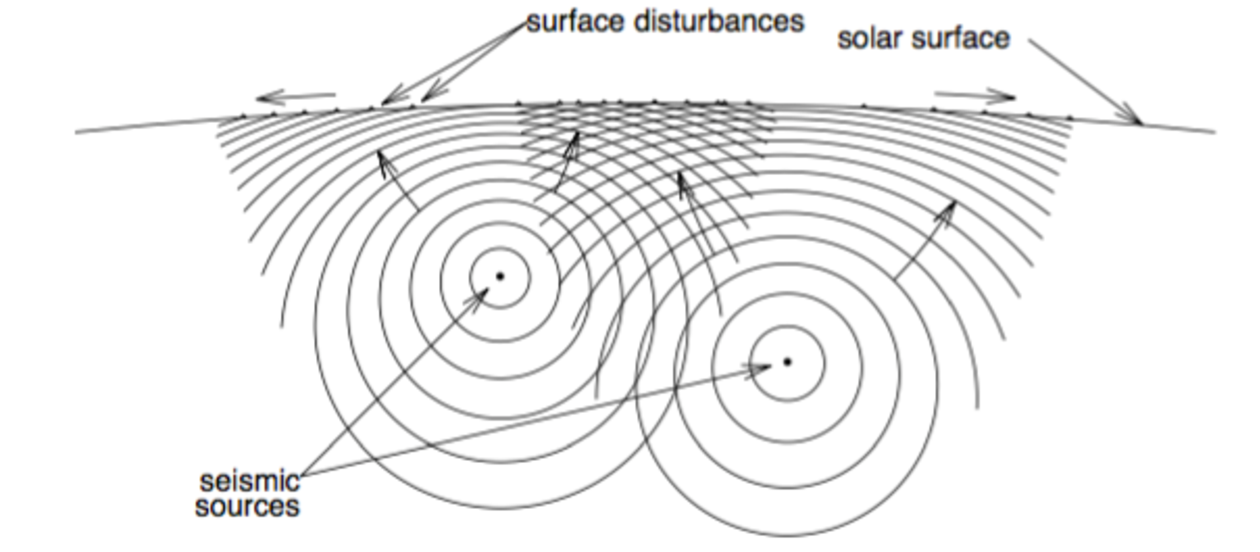
\includegraphics[width=0.8\textwidth]{fig_1.pdf}
        \caption{captiontext}
    \end{figure}
\end{frame}

\begin{frame}{2.2}
\end{frame}

%--------------------------------------------------------------%
%--------------------------------------------------------------%
\begin{comment}

\begin{frame}{Figure 2}
    \begin{figure}
        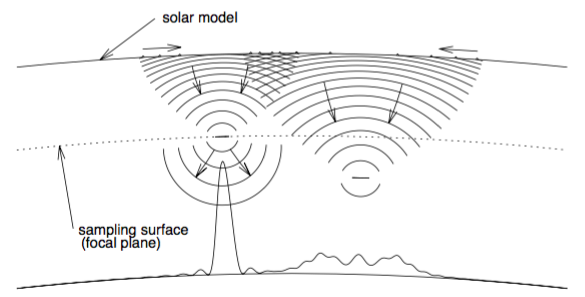
\includegraphics[width=0.8\textwidth]{fig_2.png}
       % \caption{captiontext}
       % \label{figurelabel}
    \end{figure}
\end{frame}

\begin{frame}{Figure 3}
    \begin{figure}
        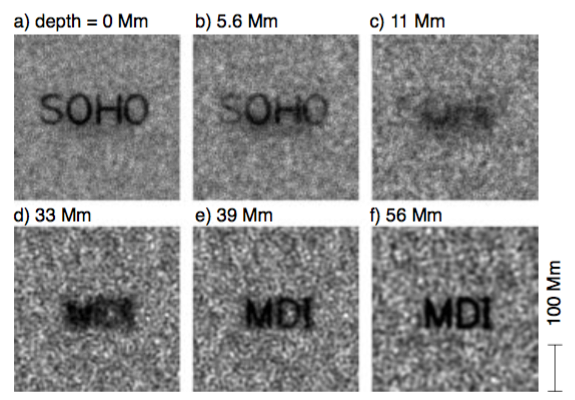
\includegraphics[width=0.8\textwidth]{fig_3.png}
       % \caption{captiontext}
       % \label{figurelabel}
    \end{figure}
\end{frame}

\begin{frame}{3. The Computational Task}
\end{frame}

\begin{frame}{Figure 4}
    \begin{figure}
        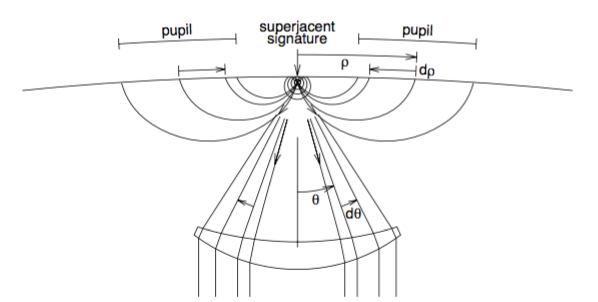
\includegraphics[width=0.8\textwidth]{fig_4.png}
       % \caption{This is figure 4}
       % \label{figurelabel}
    \end{figure}
\end{frame}

\begin{frame}{Figure 5}
    \begin{figure}
        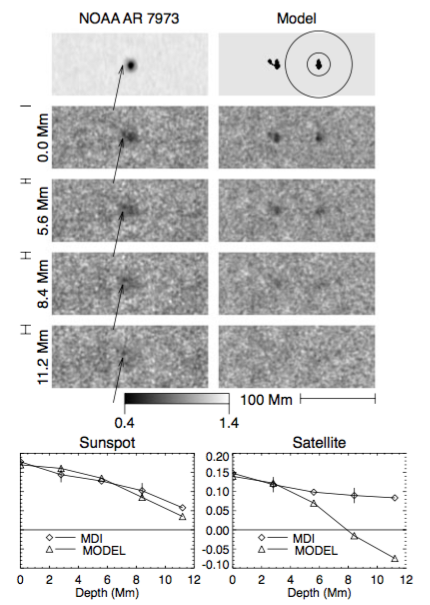
\includegraphics[width=0.8\textwidth]{fig_5.png}
       % \caption{captiontext}
       % \label{figurelabel}
    \end{figure}
\end{frame}

\begin{frame}{Figure 6}
    \begin{figure}
        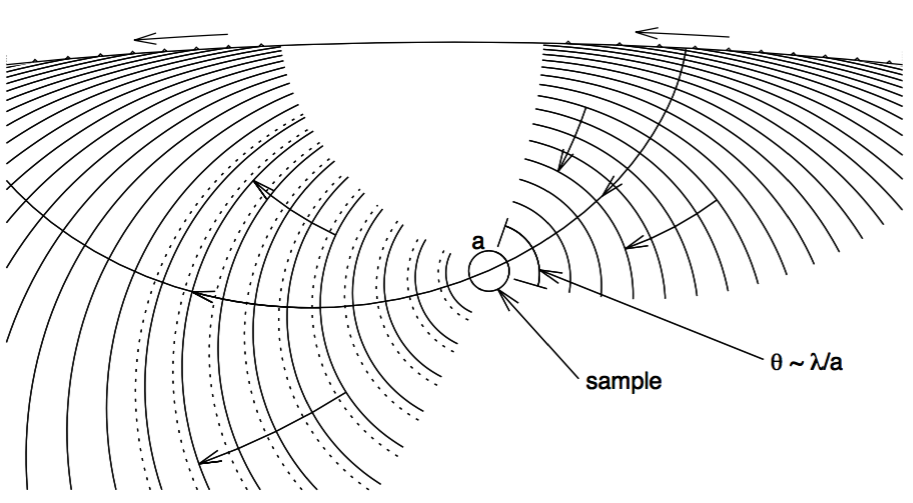
\includegraphics[width=0.8\textwidth]{fig_6.png}
        %\caption{captiontext}
       % \label{figurelabel}
    \end{figure}
\end{frame}

\begin{frame}{Figure 7}
    \begin{figure}
        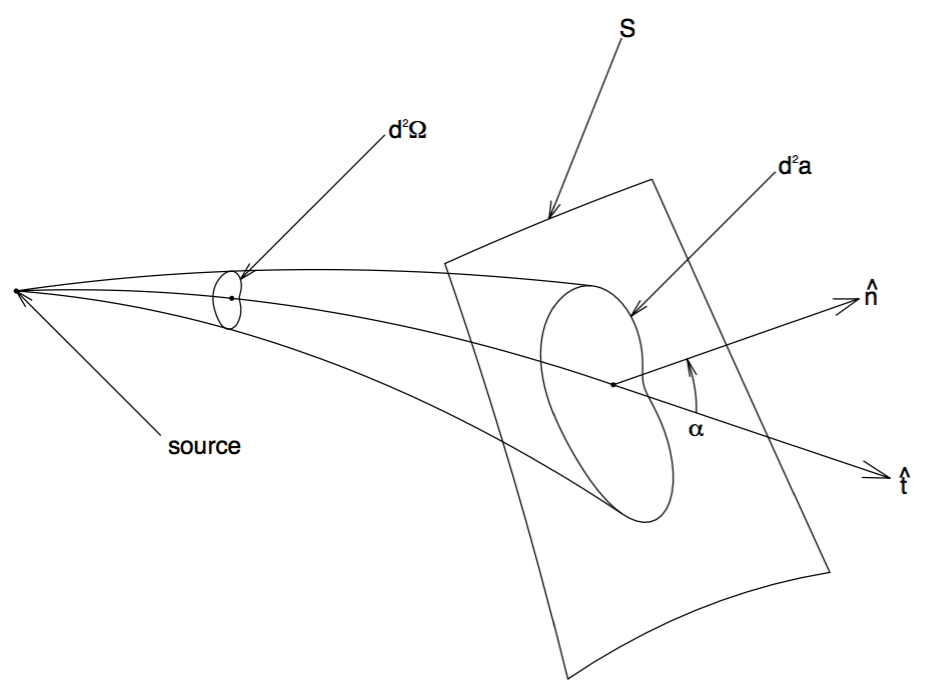
\includegraphics[width=0.8\textwidth]{fig_7.png}
       % \caption{captiontext}
       % \label{figurelabel}
    \end{figure}
\end{frame}

\begin{frame}{Figure 8}
    \begin{figure}
        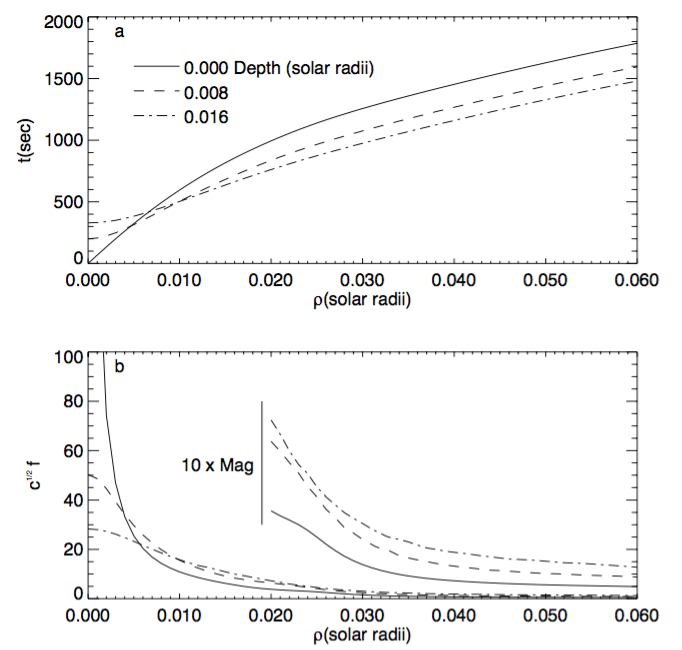
\includegraphics[width=0.8\textwidth]{fig_8.png}
       % \caption{captiontext}
       % \label{figurelabel}
    \end{figure}
\end{frame}

\begin{frame}{Figure 9}
    \begin{figure}
        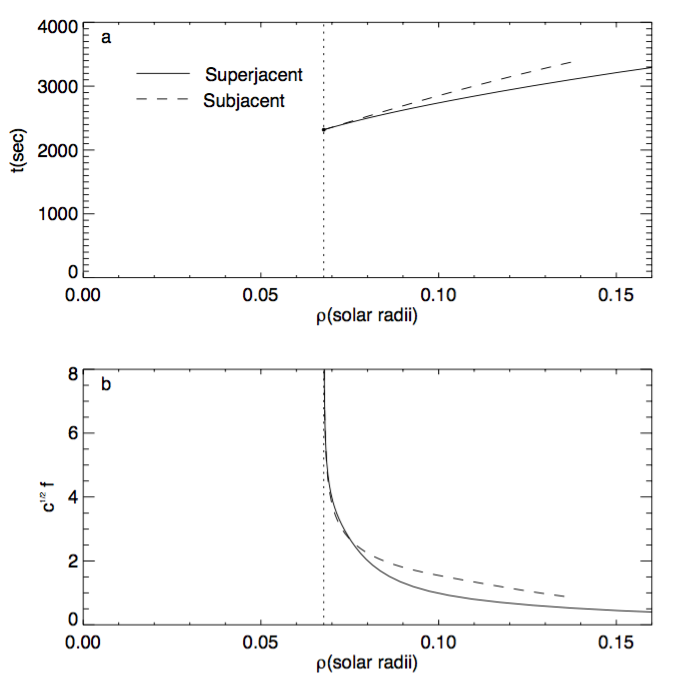
\includegraphics[width=0.8\textwidth]{fig_9.png}
       % \caption{captiontext}
       % \label{figurelabel}
    \end{figure}
\end{frame}

\begin{frame}{Figure 10}
    \begin{figure}
        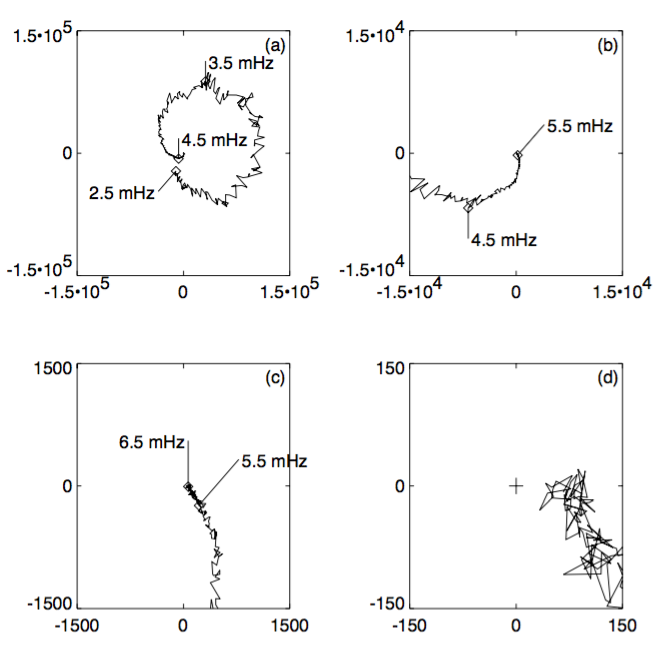
\includegraphics[width=0.8\textwidth]{fig_10.png}
       % \caption{captiontext}
       % \label{figurelabel}
    \end{figure}
\end{frame}

\begin{frame}{Figure 11}
    \begin{figure}
        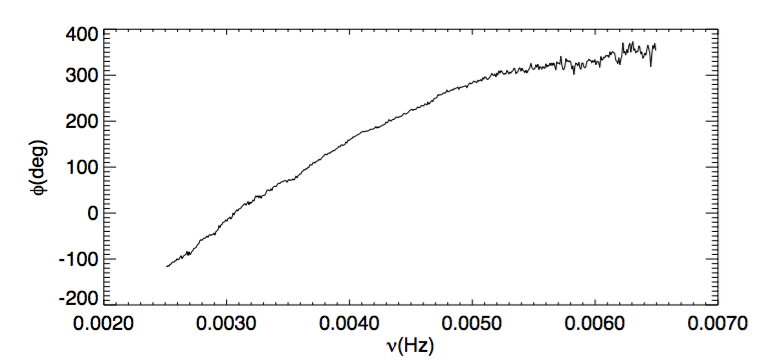
\includegraphics[width=0.8\textwidth]{fig_11.png}
       % \caption{captiontext}
       % \label{figurelabel}
    \end{figure}
\end{frame}
%--------------------------------------------------------------%
%--------------------------------------------------------------%
\end{comment}
%--------------------------------------------------------------%

\end{document}
